
\documentclass[10pt]{book}
\usepackage[width=5.5in,height=8.5in,
  hmarginratio=3:2,vmarginratio=1:1]{geometry}


% ------------------------------ 
% PACKAGES - BEGIN
% ------------------------------

\usepackage{amsthm}
\usepackage{appendix}
\usepackage[bookmarks]{hyperref}
\usepackage{color}
\usepackage{fancyhdr}
\usepackage{fancyvrb}
\usepackage{framed}
\usepackage{hevea}    
\usepackage{exercise} 
\usepackage{graphicx}
\usepackage{mathpazo}
\usepackage{makeidx}
\usepackage{setspace}
\usepackage{upquote}
\usepackage{url}
\usepackage[usenames,dvipsnames]{xcolor}
\usepackage[utf8]{inputenc}
\usepackage[T1]{fontenc}
\usepackage{textcomp} 
\usepackage{float}
\usepackage{sidecap}
\usepackage{wrapfig,lipsum} 
\usepackage{mdframed}

% ------------------------------ 
% PACKAGES - END
% ------------------------------


% ------------------------------ 
%  COMMANDS - BEGIN
% ------------------------------


\newcommand{\thetitle}{Automation with Ansible}
\newcommand{\theversion}{0.1.2}
\newcommand{\thedate}{April 2014}

\title{\thetitle}

% CSS styles for HTML  version
\newstyle{a:link}{color:black;}
\newstyle{p+p}{margin-top:1em;margin-bottom:1em}
\newstyle{img}{border:0px}

% Used for referencing with chapter/section number
\newcommand*{\fullref}[1]{\hyperref[{#1}]{\autoref*{#1} \nameref*{#1}}} 

\definecolor{NoteBackgroundColor}{RGB}{250,250,250}
\definecolor{NoteLineColor}{RGB}{216,216,216}

\mdfdefinestyle{noteStyle}{%
rightline=true,
innerleftmargin=10,innerrightmargin=10,innerbottommargin=10,innertopmargin=0,
skipbelow=5, skipabove=5,
frametitlerule=true, 
backgroundcolor=NoteBackgroundColor,%
linecolor=NoteLineColor,linewidth=1pt}

% ------------------------------ 
%  COMMANDS - END
% ------------------------------


\makeindex

\newif\ifplastex
\plastexfalse

\usepackage{eso-pic}
\newcommand\BackgroundPic{%
\put(0,0){%
\parbox[b][\paperheight]{\paperwidth}{%
\vfill
\centering

\includegraphics[width=\paperwidth,height=\paperheight%
]{figures/cover.eps}%
\vfill
}}}


\begin{document}

\frontmatter

% PLASTEX ONLY
\ifplastex
    \usepackage{localdef}
    \maketitle

\newcount\anchorcnt
\newcommand*{\Anchor}[1]{%
  \@bsphack%
    \Hy@GlobalStepCount\anchorcnt%
    \edef\@currentHref{anchor.\the\anchorcnt}% 
    \Hy@raisedlink{\hyper@anchorstart{\@currentHref}\hyper@anchorend}% 
    \M@gettitle{}\label{#1}% 
    \@esphack%
}


\else
% skip the following for plastex

\newtheorem{exercise}{Exercise}[chapter]

% LATEXONLY

\input{latexonly}

\begin{latexonly}

\renewcommand{\blankpage}{\thispagestyle{empty} \quad \newpage}

%\blankpage
%\blankpage

% ------------------------------ 
%  TITLE PAGE - LATEX VERSION - BEGIN
% ------------------------------


%-half title--------------------------------------------------
\thispagestyle{empty}

\AddToShipoutPicture*{\BackgroundPic}


%--verso------------------------------------------------------

\blankpage


%--title page--------------------------------------------------
\pagebreak
\thispagestyle{empty}

\begin{flushright}
\vspace*{2.0in}

\begin{spacing}{3}
{\huge \thetitle}\\
\end{spacing}

\vspace{0.25in}

Version \theversion

\thedate

\vspace{1in}


{\Large
Adham Helal\\
Engin Yöyen\\
}


\vspace{0.5in}


\vfill

\end{flushright}


% ------------------------------ 
%  COPYRIGHT - BEGIN
% ------------------------------

\pagebreak
\thispagestyle{empty}

{\small
Copyright \copyright~2014 Adham Helal, Engin Yöyen.


\vspace{0.2in}



Permission is granted to copy, distribute, and/or modify this document
under the terms of the Creative Commons Attribution-NonCommercial 3.0 Unported
License, which is available at 
\\
\\
\url{http://creativecommons.org/licenses/by-nc/3.0/}.

The original form of this book is \LaTeX\ source code.  Compiling this
\LaTeX\ source has the effect of generating a device-independent
representation of a textbook, which can be converted to other formats
and printed. 

The \LaTeX\ source that is used in this book is taken from \emph{Think Python} book.
\\
\\
\url{http://www.greenteapress.com/thinkpython/thinkpython.html}



% ------------------------------ 
%  COPYRIGHT - END
% ------------------------------

\vspace{0.2in}

} % end small

\end{latexonly}


% HTMLONLY

\begin{htmlonly}

% TITLE PAGE FOR HTML VERSION

{\Large \thetitle}

{\large Adham Helal, Engin Yöyen}

Version \theversion

\thedate

\setcounter{chapter}{-1}

\end{htmlonly}

\fi


% ------------------------------ 
% PREFACE - BEGIN
% ------------------------------

\chapter{Preface}

\section*{About this book}
We believe in Open-Source. And to be honest we had no great goal neither idea, when we have start it 
to write this book. We were just amazed by the technology, so we decided at work 
while we're both grabbing a coffee and talking most likely about something 
non-sense on the couch. However, we aim to make it simple, to be good enough to 
help new-comers immediately, and make it open-source because we believe in open-source.


\section*{Structure of the book}
Our approach of writing this book is to make it stable and good enough for any 
one who wants to start Ansible. From there on we want to improve and add new chapters in future, 
which also means anyone who want to write a chapter, or make a correction is welcome to do 
so. Therefore initial version will only contain several chapters, and we will 
try our best to add new chapters and make corrections.

That is being said: we do not believe reading hundred of pages and than magically start doing 
something. We think you need to get your hands dirty, and despite this might sometimes 
be the hard way to learn, we think it is the best way to learn.

Many books contains just to much unnecessary and detailed information. Beginners 
do not need the history of a technology, it is waste of time, at least this is our view. 
We believe if you are interested in minor details, history and philosophy behind 
it you can find it your own.
We want it to give the fundamentals of the Ansible, and the quickest way to 
start working with it. That is why we targeted to make short chapters that user can start and finish, 
and exercises that describe the concept of Ansible step by step.

Some of the chapters are completely based on the case studies, it means, 

\begin{itemize}
\item A task or a problem is identified 
\item Way to solve it is identified
\item An example of how to solve the problem step by step explained
\item Concept and terminology behind the example is explained
\end{itemize}

Other chapters will combine minimal amount of text and code but will not include 
any unnecessary information.

\normalsize
\clearemptydoublepage
% ------------------------------ 
% PREFACE - END
% ------------------------------



% ------------------------------ 
% TABLE OF CONTENTS - BEGIN
% ------------------------------

\begin{latexonly}
\tableofcontents
\clearemptydoublepage
\end{latexonly}

% ------------------------------ 
% TABLE OF CONTENTS - END
% ------------------------------



% ------------------------------
% ------------------------------
% ------------------------------ 
% BEGINNING OF THE BOOK
% ------------------------------



% ------------------------------
% ------------------------------
% ------------------------------ 
% Beginning of a chapter
% ------------------------------

\mainmatter

\chapter{Automaton}
Chaos and complexity: it is the part of our lives, this is especially true among 
us. By \emph{us}, I mean developers, system administrators, software engineers or what ever title we 
choose or given. We did have accepted chaos and complexity soon as we have 
started to get interested in the field of computer science and we love it, as 
much as we hate it. We build: useful, sometimes fantastic software that we are proud of it. 
It is beautiful and amazing thing, what one can do with a computer. 
We have this beautiful abstraction layer and we use other existing softwares, servers, 
libraries, and as result we can deliver a software product that helps other people, make their life easier, 
more enjoyable or make some one eventually rich. 

However we need to fix bugs, implement new features and eventually update it.
Based on our economical and business environment the software that is being 
build must be delivered frequently and process of delivery must be reliable. 
This is the part where the {\bf complexity} arises; suddenly you notice that every 
single piece of software that your application requires to function (e.g. nginx, ntp, postfix, ruby, git ). 
Well, we could count hundred more items, but you got the point. 

Most software companies, under time and financial pressure, will ignore the any sort of 
configuration that will ease up their life. We have done it many times; we will do it in future as well. 
But soon as software start to grow and you see your system-admin sweeting and trying to 
install one virtual machine after another, one update after another: 
well this is the {\bf chaos} and it is a sign that indicates time to change things and start automation.

In this book we will address the issue of chaos and complexity by 
introducing a powerful automation tool.  To be more precise, we will take a 
process that is running successfully without any problem and automated. 
In this sense main topics we will be dealing with it will be {\bf Configuration Management} 
and {\bf Continuous Delivery}.

\section{Continuous Integration \& Delivery \& Deployment}
Continuous Integration \& Delivery \& Deployment are by nature system-design practises.
These design practises are most often misused and also little bit confusing 
because of the jargon, but let us clear the air. 


\begin{description}

\item[Continuous Integration :] is the practice of frequently building a software, by 
checking out your code from code repository (e.g. Git, SVN, CVS). There are several systems which employe 
this practise such as Jenkins, Travis, Bamboo, CruiseControl. The idea behind this 
practice is to test your code often as possible (every time developer adds a new piece of code), to reduce code errors and 
increase productivity with very short development cycles. In this practise 
developer is informed immediately when tests fails, so developer can fix the 
problem quickly and commit/push changes to code repository.

\item[Continuous Delivery :] is the practice of ensuring that a software can be 
deployed to the production at any time. You can think this as an extended version of Continuous 
Integration. Software product in this stage can be under further tests which automated tests can not catch, 
such as design issues. However, the main goal is to ensure that software can be deployed rapidly. 
While Continuous Integration makes sure software is buildable, Continuous Integration 
takes the job of delivering software product, meaning deploying actually to 
servers.

\item[Continuous Deployment :] is the automation of the Continuous Delivery. 
Meaning, code that is passed thought the chain of events and passed all tests 
deployed to the production. 

\end{description}


Now, why these practises do matter? Because automation does decreases and
eventually removes the task of configuration. To see why this is such a big deal, please answer following questions:
\begin{itemize}
\item How long does it take for you to deploy a software product such as web application that your company developed?
\item In case some one else in your team need to make the deployment, how long they 
will need?
\item In case your server crashes and you need to re-configure everything, how long will this take?
\item How long do you spend to prepare documentation of system configuration?
\end{itemize}

Imagine that you could execute a single command and that will take care of installing dozens of 
dependencies and several hours of server configuration. This is all possible, it 
is not new, neither a rocket science, and we are hoping to show you all with Ansible to prove a point
how easy it is. That is why this practises do matter,
and you should very much prefer to use your time for something valuable 
(such as drinking coffee on couch) than making server configuration.


\section{Configuration Management}
Configuration management is a process of configuring basic OS 
services and enforcing their state across IT infrastructure, however this is not 
limited to OS services and can be extended to services such as setting up an HTTP server (e.g. 
Apache). The goal here is to have several blueprints based on your infrastructure, 
for instance having one blueprint for your web servers and one for your database servers. Let us assume that
you have twenty web servers and four database servers. The goal here is to when 
ever you make a change in a blueprint, such as web servers blueprint, this is applied 
across all web servers. So to say, all of your servers are in same state, 
without someone manually making change in every single of them.

 
\section{Orchestration}
We are way beyond the time, where we once knew where the heck is our server. 
Now days we have cloud, we have servers all around the globe, and we have hundreds of them. 
This is the point where orchestration comes into play. 
Orchestration describes the process where group of automated tasks are executed, 
coordinated and managed. Why the fancy word? 
To begin with, it sounds good, on the other hand, this fancy word and concept will reduce 
all the errors that you are making while updating your 
software stack and watching TV at the same time. it will give you automation 
capability way beyond imagination. 



\section{Ansible}
\subsection{What is Ansible?}
Ansible is open-source automation and orchestration engine. In other words, 
it includes all necessary IT automation tools. It is a very simple yet powerful tool to use: 
it does not requires hours long setup for managing your servers, it is scalable, 
it is secure, it is easy to understand.


\subsection{How does it work?}
Ansible works by connecting your remote servers via SSH, and will push out 
small programs which are executed by Ansible. 
These small programs will be the desired state of the infrastructure configuration.
Ansible then executes these programs over SSH and deletes them when finished.


\subsection{Why SSH?}
Using SSH brings many features out-of-the-box and solves bucket-load of 
problems. Here are few of them:

\begin{itemize}
\item Agentless : No server-side software or agent required, you only need OpenSSH 
daemon.
\item Secure: It is a very secure protocol.
\item Resource Utilization: When Ansible is not managing remote server there 
are no resources consumed on those servers.
\item Turn-Key: Allows you to start managing your machines immediately.

\item Credential Segregation: It uses existing SSH credentials, as well as your 
privileges. For instance, if a developer is not allow to access to production server 
he will not be able to push contents to that server.
 
\end{itemize}
 
 


\subsection{How to use it?}
Using Ansible is pretty straight forwards actually, however you should posses some knowledge 
of :

\begin{itemize}
\item SSH and basic bash
\item Working with the command line
\item Perform basic maintenance tasks
\end{itemize}

We think at least you should have some of the knowledge that is in the scope of 
The Linux Professional Institute Certification(LPIC-1) first level.
Read about LPIC at 
\\
\\
\url{http://en.wikipedia.org/wiki/Linux_Professional_Institute_Certification}

 
\section{To Get Started}
\label{sec:to-get-started}
We did not want it to have installation details of tools to became main body of the book, therefore 
we have added these kind of information into appendices. Under each section, you 
will find relevant information that you will need it, 
which in case of installation details you will be referred it to relevant appendix. 


\subsection{How to install it?}
Please refer to  \emph{Appendix \fullref{appendix:How-to-install-ansible}} for 
installation details. If you have already installed Ansible you can skip this 
section.

\subsection{Using a Vagrant Machine}
\label{sec:using-vagrant-machine}
 This section is for those who does not have any idea about how to use 
virtual machines. 

You need to get your hands dirty, so you need an environment to test things you 
learn. Therefore we encourage you to start testing while you are reading it. To solve 
to test-server problem, we suggest you to use Vagrant.
Vagrant is a tool for creating, configuring, managing virtual 
machines\footnote {\url{http://www.vagrantup.com/}}.
We have prepared a simple Vagrant file which you can use 
for firing one or several virtual machines quickly. 

Please refer to \emph{Appendix \fullref{appendix:installing-and-using-vagrant}} for 
installation details. If you have already installed Vagrant and you know how it works you can skip this 
section.


\subsection{Where are the source files?}
\label{sec:book-source-codes}
You can find the source code of examples that are given in this book 
in the same repository as this book:

\url{https://github.com/AutomationWithAnsible/book}

Under folder \emph{source-code} you can find the examples that corresponds to 
chapter number and name.

\section{Up Shot}
In this chapter we have introduced software delivery and configuration practises 
and we have introduced Ansible:

\begin{itemize}
\item Continuous Integration : is the practice of frequently building a software and running tests against 
your source code to validate the functionality that has been developed.

\item Continuous Delivery : is the practice of deploying software rapidly and 
automatise fashion without any developer involvement.

\item Continuous Deployment : is the automation of the Continuous Delivery. 

\item Configuration Management : is a process of configuration of basic OS 
services and enforcing their state across IT infrastructure. 

\item Orchestration : is a process where group of automated tasks are executed, 
coordinated and managed.

\item Ansible :  is an open-source IT automation and orchestration engine.

\end{itemize}


% ------------------------------
% End of chapter
% ------------------------------
% ------------------------------ 
% ------------------------------





% ------------------------------
% ------------------------------
% ------------------------------ 
% Beginning of a chapter
% ------------------------------


\chapter{The Good Old Command Line Interface}
We have this senseless discussion, whether Graphical User Interface(GUI) or Command Line Interface(CLI) is better. 
At the end of the argument we both agree that they have 
different purposes and somethings just does not make sense doing with GUI and 
other things with CLI. But we get back to discussion quite often. Long story short, CLI is handy, 
especially for a System Administrator or a Developer. 

In this chapter we will introduce Ansible Ad-Hoc Commands, which is a tool that might be useful for 
running some quick arbitrary commands. The actual goal is to get you up to speed 
and start using Ansible as well as explaining some basics.


\section{To Start}
Along this book, when ever you execute a code and you have a connection problem, 
first thing to check is your SSH connection. Ansible relays on SSH so it is better to understand it and
figure out why it is not connecting. Most of connection issues are:

\begin{itemize}
\item Network issues : connectivity or DNS problem
\item SSH connection issues (e.g. port, username/password, key) 
\end{itemize}

A good way to find what is the error is to eliminate them one by one, therefore try to:
\begin{itemize}
\item Ping your target hostname or IP to see whether you get any respond
\item If your target is responsive use normal ssh to verify your access
\item Check SSH username that you are connecting. Common problem is that you are 
accessing the system with wrong SSH user, for instance some system prohibits root 
ssh user login.
\item Check whether your server requires key or password based authentication
\item Check whether your user have sudo rights, it might be required based on type of operation
\item Last, you can pass the \emph{-vvvv} argument to ansible which will print out some useful info 
including connection issues
\end{itemize}

If you have regular SSH connection from terminal that it is great, you are ready to go.


\section{First Ad-hoc Commands}
Well, it is a command line argument, so it is not that complicated. Depending on your installation 
ansible will have executable file called \emph{ansible}, which is the program you 
can use for executing ad-hoc commands. For instance, here is a really basic example of how to ping a server.

\begin{Verbatim}

ansible -i 192.168.56.150, -m ping all

\end{Verbatim}


 % ---- NOTE BEGINS ---- 
\begin{mdframed}[style=noteStyle]
\begin{minipage}[b]{0.05\textwidth}
\begin{figure}[H]

\includegraphics[width=0.9\textwidth]{figures/notes-icon.eps} 
\end{figure}
\end{minipage}  
\begin{minipage}[b]{0.05\textwidth}
\textbf{Note}
\end{minipage}

IP address in this example is a server that you need to connect. If you do not 
have any server that you can test please refer to \emph{Appendix \fullref{appendix:installing-and-using-vagrant}}
\end{mdframed}
 % ---- NOTE ENDS ---- 


In the example above \emph{-i} means inventory, this is where you specify your target server. 
You can also specify more than one server by adding them after comma (,). The \emph{-m} stands for module name, 
meaning module that will be executed is the \emph{ping} module. We will be using modules a lot and in
next chapter we will already start to dive in with more detail. The \emph{all} 
refers to all hosts, meaning command will be execute on all target servers, 
but we are using only one host for now. When the code above is executed you will see the following response from your 
command line.


\begin{figure}[ht]
	\centering
  
\includegraphics{figures/first-ad-hoc-command.eps}
	\caption{Response From First Ad-hoc Command}
\end{figure}


Assumption is that you are using standard SSH port (22), if you have anything 
other than that you can specify that as well after IP address:

\begin{Verbatim}

ansible -i 192.168.56.150:24350, -m ping all

\end{Verbatim}



When you are executing ad-hoc commands by default \emph{command} module is selected, 
which you do not need to declare, this module executes commands on remote servers. You can see that from 
following example. When you execute an ad-hoc command you can pass arguments to the module. For this 
purpose you can use the \emph{-a}  and give the arguments which will pass to 
module afterwards. In this case we want \emph{whoami} command to be executed on server so 
we give that as an argument.

\begin{Verbatim}

ansible -i 192.168.56.150, -a "whoami" all

\end{Verbatim}

And response we get from server will be:


\begin{figure}[ht]
	\centering
  
\includegraphics[width=0.6\textwidth]{figures/command-execution-whoami.eps}
	\caption{Server Response to \emph{whoami}  Command}
\end{figure}


There are several other arguments you can add while executing \emph{ansible}  
command, instead of giving example of each of them, we will explain them 
briefly but only relevant ones. Short and long names are giving together:

\begin{description}
\item[-m, --module-name:] Module name to execute
\item[-a, --args:]  Module arguments
\item[-s, --sudo:]  Run operations with sudo 
\item[-k, --ask-pass:] Ask for SSH password
\item[-K, --ask-sudo-pass:] Ask for sudo password
\item[-u, --user:] Connect remote target with different user name
\item[-f, --forks:]  Specify number of parallel processes to use when communicating with remote hosts 
(default is 5)

\end{description}

\section{Examples}
Following examples are relatively minor and do not bring anything newer than 
what we have explained above, however it is good practice to start with them to 
get use to it. If you already feel comfortable with this, you can skip it to 
next section already.

\subsection{Copying File}
For copying file you will use \emph{copy} module, this module will copy a file 
from source (your machine) to a destination (provisioned machine). 

\begin{Verbatim}

ansible -i 192.168.56.150, -m copy -a  
  'src=myfile dest=/tmp/mynewfile.txt' all
 
\end{Verbatim}

In this example, as you can see argument that is passed to the module are parameterized. Meaning, source and 
destination of the file are being passed to the module. What this tell us is 
that, we can send more than one parameter to the module. For example, it is 
possible to set the file owner and mode.

\begin{Verbatim}

ansible -i 192.168.56.150, -m copy -a  
  'src=myfile dest=/tmp/mynewfile.txt mode=644 owner=jane' all
  
\end{Verbatim}

\subsection{Managing Packages}
Following example, will demonstrate usage of \emph{apt} module, which will 
make sure that latest version of nginx HTTP server is installed.

\begin{Verbatim}

ansible -i 192.168.56.150, -s -m apt -a  'pkg=nginx state=latest' all

\end{Verbatim}

Following example, will update the cache meaning it will resynchronize the package 
index.

\begin{Verbatim}

ansible -i 192.168.56.150, -s -m apt -a 'update_cache=yes' all

\end{Verbatim}

\subsection{Downloading Files}
Following example, will demonstrate usage of \emph{get\_url} module, which downloads a file 
from remote server to your target server. It support HTTP, HTTPS, and FTP 
protocols. In this example we will give two parameters, url, which is the URL 
path of the file that we want to download, and dest which is the location where 
should be saved in target host.


\begin{Verbatim}

ansible -i 192.168.56.150, -s -m get_url -a 'url=http://apache.imsam.info/
          tomcat/tomcat-8/v8.0.3/bin/apache-tomcat-8.0.3.tar.gz 
          dest=/tmp/apache-tomcat-8.0.3.tar.gz' all

\end{Verbatim}

Additionaly you can also give SHA-256 checksum of the file, to make sure file is 
downloaded correctly. Which is a useful feature for many file operations.



\section{To Learn More}
It is great to use the modules, and you will be using them for everything when 
you are writing playbooks. However, you can not learn all the modules, and all 
the parameters they accept, but you can find it out easily. To get detailed 
account of an module you can use \emph{ansible-doc} command and name of the 
module. When you execute the following command you will get complete the documentation 
of the module.


\begin{Verbatim}

ansible-doc copy

\end{Verbatim}

In Figure ~\ref{fig:ansible-documentation-output} 
on page~\pageref{fig:ansible-documentation-output} you can see the partial 
output of this command.

\begin{figure}[ht]
	\centering
  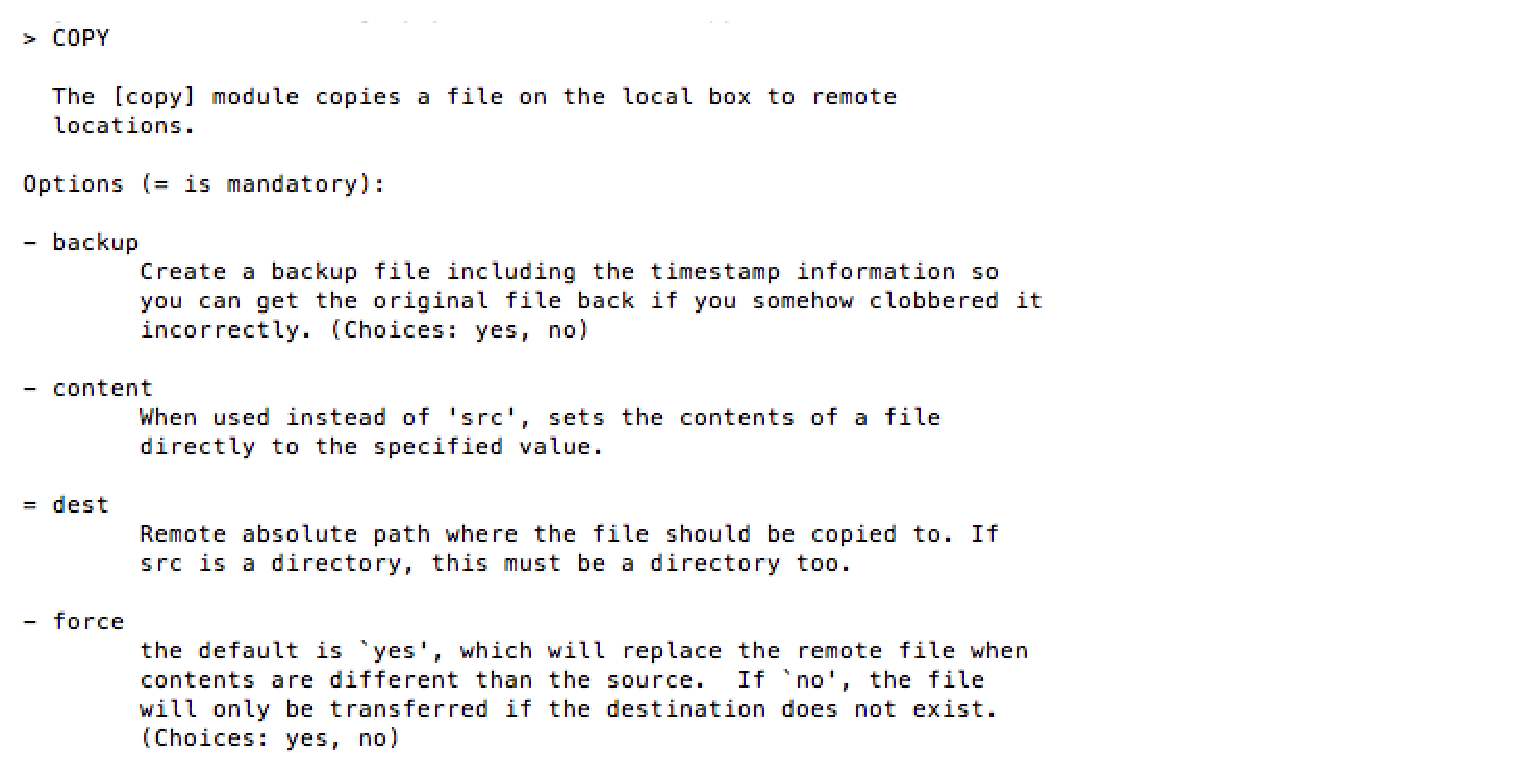
\includegraphics[width=1.0\textwidth]{figures/ansible-doc-copy.eps}
	\caption{Ansible Documentation Output}
		\label{fig:ansible-documentation-output}
\end{figure}

One other command that may help you to speed up is to learn available modules:

\begin{Verbatim}

ansible-doc -l

\end{Verbatim}

\section{Up Shot}
In this chapter, we have introduced the ad-hoc commands which laid down the 
fundamentals for working with playbooks. Now you should have understanding of executing different modules, 
how to find them and use their parameters. This information will be quite 
valuable in next chapters.



% ------------------------------
% End of chapter
% ------------------------------
% ------------------------------ 
% ------------------------------




% ------------------------------
% ------------------------------
% ------------------------------ 
% Beginning of a chapter
% ------------------------------


\chapter{Case Study : Common Post Installation Setup}
\label{chap-common-post-installation-setup}
To begin with, we are going to do very simple exercise, which we will take over some of the basics from 
last chapter and develop on top of it. Furthermore, we will explain some of the key concept of Ansible in 
this chapter.

\section{The Problem}
Here is our problem:

\begin{quote}
 We have a fresh installed \emph{Ubuntu Precise 12.04}. Now, the first thing we need to do after installation 
 is to upgrade and patch the system. This is a good practice because the system will be 
 up-to-date, meaning fewer bugs, less security issues. Afterwards we want to change the 
 hostname, because it will be easy to identify to server. Next step is to install 
 Network Time Protocol (NTP); this will help our system time to be synchronized. 
\end{quote}

In other words, here are the steps:
\begin{itemize}
\item Update the apt repository: Updates the package management repository
\item Upgrade the packages: Upgrades the existing software packages (e.g. security, apache), 
removes some of the packages and keep dependency
\item Upgrade the kernel 
\item Change the host name
\item Install NTP
\end{itemize}

This is a relatively simple example of {\bf Common Post Installation Setup}, 
which can be extended to any range, but we will keep it simple for now. 

\section{Requirements}
For completing this chapter following list should be completed;
\begin{itemize}
\item Server that is up and running 
\item Your public SSH key installed on remote server
\item Ansible is installed on your computer
\end{itemize}

 % ---- NOTE BEGINS ---- 
\begin{mdframed}[style=noteStyle]
\begin{minipage}[b]{0.05\textwidth}
\begin{figure}[H]

\includegraphics[width=0.9\textwidth]{figures/notes-icon.eps} 
\end{figure}
\end{minipage}  
\begin{minipage}[b]{0.05\textwidth}
\textbf{Note}
\end{minipage}

If you do not have any server that you can test, please refer to \emph{Appendix \fullref{appendix:installing-and-using-vagrant}}
\end{mdframed}
 % ---- NOTE ENDS ---- 
 


\section{Playbook}
In problem description, we have showed a road map of how to accomplish the tasks, one by one.
Under normal circumstances what you will do is, you will complete the tasks with 
certain order or you will put them all in a some bash script file and execute 
it. It will definitely do the trick, but it won't be enough. This is where Ansible 
comes into play; Ansible introduced a concept called {\bf playbooks}, which is a simple text file that 
describes configuration, a policy or a set of steps which can be used to 
configure a remote server. Playbooks are very powerful and very 
simple; they are expressed in YAML format, which is human-readable data serialization 
format \footnote { \url{http://en.wikipedia.org/wiki/YAML}}. 

 % ---- NOTE BEGINS ---- 
\begin{mdframed}[style=noteStyle]
\begin{minipage}[b]{0.05\textwidth}
\begin{figure}[H]

\includegraphics[width=0.9\textwidth]{figures/notes-icon.eps} 
\end{figure}
\end{minipage}  
\begin{minipage}[b]{0.05\textwidth}
\textbf{Note}
\end{minipage}

A fair warning:  YAML relies on outline indentation 
for structure which makes sometimes hard to type things quick and dirty way. 
Therefore we suggest that you use a good text editor with auto-intentation support, otherwise you will
be spending a lot of time correcting indentation manually.
\end{mdframed}
 % ---- NOTE ENDS ---- 


Now, let's create our first playbook. Create a new text file, and save it under the name 
\emph{common-post-installation.yml}, under a directory of your choice. For 
Ansible, most of the playbooks starts with a list, and each item in the list is a list of key/value 
pairs. Here is our first playbook, that contains just a one play:

 % Used to start code in next page
\vspace{10 mm}
 
\begin{Verbatim} 
 
---
# This playbook play all post common installation for all servers

- hosts: all
  sudo: True

  tasks:
    - name : Update apt cache
      apt  : 
         update_cache=yes

    - name : apt upgrade
      apt : 
         upgrade=yes

    - name : apt dist
      apt : 
         upgrade=dist

    - name: Change hostname
      hostname: 
         name=web01

    - name: install ntp
      apt:  
         pkg=ntp
         state=present

\end{Verbatim}
 
The three dash at the top of the file indicates the beginning of the file, this is YAML syntax. 
The {\bf hosts} line holds the target group, meaning which servers we want this playbook to run.
In each playbook, there can be more than one play, meaning group of hosts can be tided up to certain 
tasks. For the sake of simplicity, we gave the value {\bf all} to parameter {\bf hosts}, 
in next chapter we will use other examples, where we will be using hosts declaration.

The {\bf tasks} line holds the list of tasks that we want it to be accomplish 
in order and they are executed in order, one at a time, 
against all machines that are specified. Each task has a 
name and job to execute a module with a specific argument. 
The name in each task will be used in the output, it is a good 
practice to give names, we suggest that you do it as well. In our playbook we 
are using two modules \emph{apt} and \emph{hostname}, which manages apt-packages 
and changes the hostname respectively. In this example we use different 
arguments against same module, such as updating cache and upgrading. This 
arguments are very well documented, which in the following chapters we will get 
back to it again. 

Now it is time to execute the tasks. For 
executing playbooks we will be using \emph{ansible-playbook}.

\begin{Verbatim} 

ansible-playbook -i 192.168.56.150,  /[FilePath]/common-post-installation.yml 
  
\end{Verbatim}

Soon as you execute the code, you should see that ansible start working, and you 
will see the output. Output will give you details of the tasks whether succeeded, 
any-change has been made or failed. If one of the tasks is failed while running a play, 
you can solve the problem and re-run the play. Here is how the console output should look like:


\begin{figure}[ht]
	\centering
  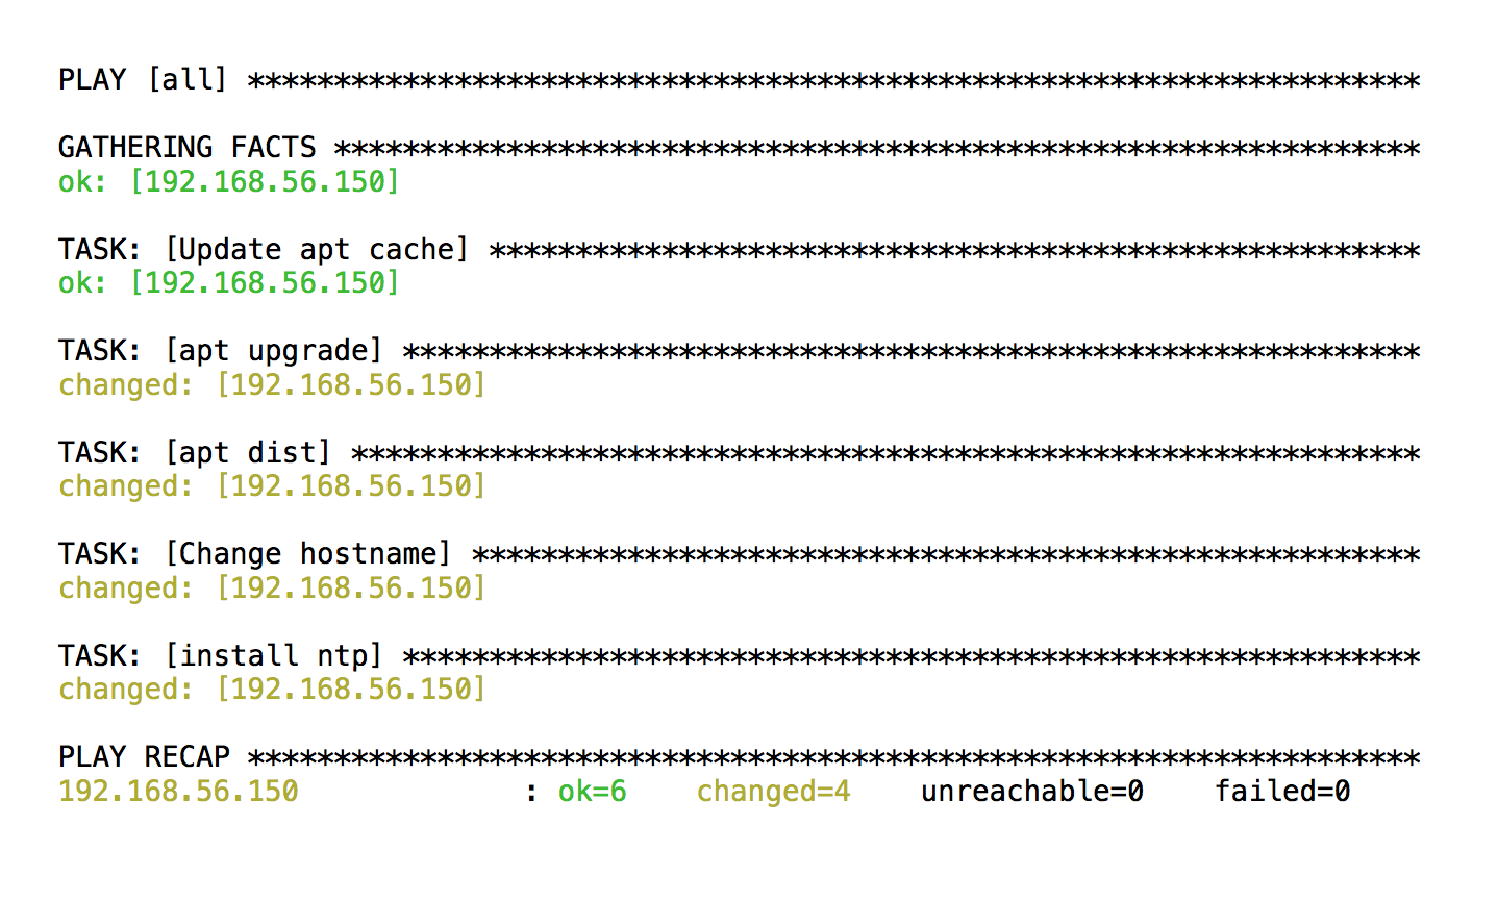
\includegraphics[width=1.0\textwidth]{figures/common-post-installation-output.eps}
	\caption{Common Post Installation Output}
\end{figure}

In case of re-running a play, all tasks will run from top to bottom. As we have 
explained before, the goal is to bring a system to the desired state, in re-run, 
tasks that were successful \textbf{will-not} make any changes in the system again, 
meaning they will only make the changes that are required to bring the system to the desired 
state. This allows multiple execution of same play. To try out this, what you 
can simply do is, after your play runs once successfully, re-execute the command 
and watch the output. Result you get will be \textit{OK}, but there won't be 
any changes. This is called \textbf{idempotent}, meaning change commands are not run unless 
needed \footnote {\url{http://en.wikipedia.org/wiki/Idempotence}}. So to say, every-time you execute this play, system will not install 
NTP.



 % ---- NOTE BEGINS ---- 
\begin{mdframed}[style=noteStyle]
\begin{minipage}[b]{0.05\textwidth}
\begin{figure}[H]

\includegraphics[width=0.9\textwidth]{figures/notes-icon.eps} 
\end{figure}
\end{minipage}  
\begin{minipage}[b]{0.05\textwidth}
\textbf{Note}
\end{minipage}

You could write all your modules arguments in one line as you can see in this example. 
However code format that we will follow in this book is to use new line for every argument 
as in previous play.

\begin{Verbatim} 
    - name: install ntp
      apt: pkg=ntp state=present
\end{Verbatim}

\end{mdframed}
 % ---- NOTE ENDS ---- 



\section{Troubleshooting}

\begin{itemize}
\item No response from Ansible or stucks after \textit{GATHERING FACTS} message.

Most likely hanged while waiting for sudo password, to solve it, add following argument 
\begin{Verbatim}
--ask-sudo-pass  or -K
\end{Verbatim}
and it will ask the sudo password.

\item SSH encountered an unknown error during the connection message

Check your server whether is running or not, check your connection via 
terminal to establish a SSH connection
\end{itemize}


\section{Up Shot}
In this chapter, we have made a very simple example, which introduce the 
following concepts:

\begin{itemize}
\item Tasks : List of actions that you want to be taken in remote server
\item Playbook : Configuration management file, that holds all relevant 
information to achieve the desired state on your system
\item Modules : A tool to accomplish a certain task
\end{itemize}

For finding source code of this example please refer to \emph{\fullref{sec:book-source-codes}}

In next chapters we will dig into all these concepts one by one with more 
details and examples.

% ------------------------------
% End of chapter
% ------------------------------
% ------------------------------ 
% ------------------------------

 
 
% ------------------------------
% ------------------------------
% ------------------------------ 
% Beginning of a chapter
% ------------------------------


\chapter{Case Study : Deploying Web Application with Nginx}
\label{chap-deploying-web-application-with-nginx}
In this chapter we will show very basic example of how you could deploy an 
simple web application. Furthermore, we will explain some basic concepts such as 
variables, loops, templates and handlers that will be very useful for future 
playboo deployment.


\section{The Problem}
Here is our problem:

\begin{quote}
We do have a PHP web application and we want to deploy on a server. Naturally, we need a web server
which will be the nginx, this also means there will be some server 
configuration.
\end{quote}

In other words, here are the steps:
\begin{itemize}
\item Install nginx web server 
\item Install  PHP-FPM
\item Apply configuration
\item Copy web application to remote machine
\item Restart nginx
\end{itemize}

So it is a relatively simple task, but do not worry, we will introduce some new 
things as well.

\section{Variables}
It is most likely that you will face a situation that some of your server should 
behave or do something different than others despite they might be all classified as web servers. 
For instance, you may have a bunch of development servers which one of them is public and 
you want some special rights to be applied for that server. In such a case 
setting variables for particular host or a group might be really useful. 
These custom variables can be used easily by playbooks. In our example, we will 
have two configuration files, one of them is nginx configuration file, and the 
other one default configuration file of the web application. Both of these files 
will have some variables, that we want it to replace it. For time being, we will define 
variables in playbooks. There are other ways to do that, but for now we will 
take a simple approach. In playbook, you can define the variable like this:

\begin{verbatim}

---
- hosts: all
  sudo: True
  vars:
    delete_default_vhost: false
    user: www-data
    worker_processes: 4 
    pid: /var/run/nginx.pid
    worker_connections: 768
    httpPort: 80

\end{verbatim}
 
As you see it is relatively simple, everything under \emph{vars} are treated as 
variable and available to be used for templates and tasks.

\section{Templates}
As we have mentioned, we have two configuration files, which we want these variables to be injected in them.
For this purpose Ansible uses Jinja2 templating system, which is a designer friendly templating language 
for Python, modelled after Django’s templates\footnote { \url{http://jinja.pocoo.org/docs/}}.
For referencing a variable you have to put double curly braces around the variable 
name. Here is a simple example of how should it look like:

\begin{verbatim}

{{worker_connections}} 

\end{verbatim}

\subsection{Template Files}
We will be using variable references in \emph{.j2} file(a text file) which we will deliver to 
the server. In this case we will have a template file, which will be structured 
in a way that we want it to be deliver. Values that we do want to be dynamic will be replaced with 
variables names with double curly braces around. As you can see from following 
example, variables that are defined in playbook are used in template file. 
Here is the nginx configuration file, called \emph{nginx.conf.j2}:

\begin{verbatim}

user {{ user }};
worker_processes {{ worker_processes }};
pid {{ pid }};
events {
    worker_connections {{ worker_connections }};
}

http {
    # Basic Settings
    sendfile on;
    tcp_nopush on;
    tcp_nodelay on;
    keepalive_timeout 65;
    types_hash_max_size 2048;

    include /etc/nginx/mime.types;
    default_type application/octet-stream;

    # Logging Settings
    access_log /var/log/nginx/access.log;
    error_log /var/log/nginx/error.log;

    # Virtual Host Configs
    include /etc/nginx/conf.d/*.conf;
    include /etc/nginx/sites-enabled/*;
}

\end{verbatim}

So what we accomplish here is having a static file, which content will be determined based on 
variables that are injected in. And here is the web application configuration file, called \emph{default.j2}:

\begin{verbatim}
  
server {
       listen   {{httpPort}}; 
       listen   [::]:{{httpPort}} default ipv6only=on; 

       root /usr/share/nginx/www;
       index index.html index.htm;

       server_name localhost;

       location / {
              try_files $uri $uri/ /index.html;
       }
       
       location ~ \.php$ {
              try_files $uri =404;
              fastcgi_pass 127.0.0.1:9000;
              fastcgi_index index.php;
              include fastcgi_params;
      	}
}

\end{verbatim}

 % ---- NOTE BEGINS ---- 
\begin{mdframed}[style=noteStyle]
\begin{minipage}[b]{0.05\textwidth}
\begin{figure}[H]

\includegraphics[width=0.9\textwidth]{figures/notes-icon.eps} 
\end{figure}
\end{minipage}  
\begin{minipage}[b]{0.05\textwidth}
\textbf{Note}
\end{minipage}

You do not have to understand the nginx configuration, it is just an example 
that we are using here.

\end{mdframed}
 % ---- NOTE ENDS ---- 
 
\subsection{Template Module}
We have now templates files and variables, only thing that is left is to use the 
template module to transfer configuration files from source to destination. As 
you can see from the following example, for this purpose we are using \emph{template} 
module and we specify the source file, which is the template file and the 
destination. 

\begin{verbatim}

- name: write nginx.conf
  template: 
     src=nginx.conf.j2
     dest=/etc/nginx/nginx.conf
         
\end{verbatim}

Variables that are defined in template file will be replaced by real values 
without further work. As a result, destination server will have file called 
\emph{nginx.conf} and all variables are replaced with real values.


\section{Loops}
In previous chapter we have explain how you can install a software package on a 
server. As you will remember it, it was relatively simple, in this example we have two dependencies, one 
of them is \emph{nginx}, which is the http server, the other one is \emph{php5-fpm}, which is the dependency
required to run PHP application. If we want to write the code that will make the installation of these 
dependencies code should look like this (based on what we 
have shown in previous chapter) :

\begin{Verbatim} 

- name: Install nginx  
   apt:
     pkg=nginx 
     state=present"

- name: Install php-fpm 
   apt:
     pkg=php5-fpm
     state=present"

\end{Verbatim}

This code is completely functional without any error. In this example there are 
only two dependencies so writing code for it is quick. However when you have dozens of 
them in one play duplicating line after line is not productive. Doing many 
similar tasks one after the other, such as package installation, user creation 
or copying file is a repeated tasks, and it is not efficient to copy and paste.

For this purpose you can use loops. A loop is a sequence of statements which is specified 
once but which may be carried out several times in succession\footnote {\url{http://en.wikipedia.org/wiki/Loop_(computing)\#Loops}}. .
Following is a standard loop, which you can specify a list with \emph{with\_items} directive 
and give the variable reference \emph{item} to the \emph{pkg} argument as 
parameter. This code is equivalent as one above.

\begin{Verbatim} 

- name: Install nginx and php-fpm 
  apt: 
     pkg="{{item}}" 
     state=present
  with_items:
     - nginx
     - php5-fpm

\end{Verbatim}

 % ---- NOTE BEGINS ---- 
\begin{mdframed}[style=noteStyle]
\begin{minipage}[b]{0.05\textwidth}
\begin{figure}[H]

\includegraphics[width=0.9\textwidth]{figures/notes-icon.eps} 
\end{figure}
\end{minipage}  
\begin{minipage}[b]{0.05\textwidth}
\textbf{Note}
\end{minipage}

Specifying list of items is also possible with traditional array structure :

\begin{Verbatim} 
- name: Install nginx and php-fpm 
  apt: 
     pkg="{{item}}" 
     state=present
  with_items: 
    ["nginx","php5-fpm"]
\end{Verbatim}

\end{mdframed}
 % ---- NOTE ENDS ---- 
 


Because our web application will have some files and we have to copy them to the 
server, for this purpose we can use loops for copying files as well:

\begin{Verbatim} 

- name: Copy files
  copy: 
     src="{{item}}"
     dest="/usr/share/nginx/www/{{item}}"
  with_items:
     - index.html 
     - myapp.php

\end{Verbatim}



\section{Handlers}
Now we know how to install nginx, copy files and make the configuration files based on variables and templates. 
But we also need to restart the server because we do change the configuration of 
the server. Despite there are many way to do this kind of actions, best way to 
go is to use something easy and simple: \emph{handlers}. In ansible handlers are just list of 
tasks, like others, difference is that for a task to be executed handler have to 
be notified. Let's give an example for this: following handler 
will restart the nginx when it is being notified by a task. In the example below 
when template module completes it's job it notifies the handler. The \emph{notify}
directive contains the name of the handler.

\begin{Verbatim} 

tasks:  
    - name: write nginx.conf
      template: 
         src=nginx.conf.j2
         dest=/etc/nginx/nginx.conf
      notify:
         - restart nginx
     
handlers:
    - name: restart nginx
      service: 
         name=nginx
         state=restarted
         enabled=yes

\end{Verbatim}

The \emph{notify} directive registers an change event and informs the handlers. 
If there are no changes there are no triggers.

In the example above, \emph{service} module, controls daemon on remote hosts. 
The parameter \emph{state} in this case is set to \emph{restart}, meaning it will always restart the nginx.
The parameter \emph{enabled} means service is enabled on boot.

The beauty of handlers is that they could be notify \emph{n} time, but they will be 
executed only ones after all tasks are completed in a play.


\section{Putting it Together}
Now here is the complete play with variables, template module, loops and handlers.

\begin{Verbatim} 

---
- hosts: all
  sudo: True
  vars:
    delete_default_vhost: false
    user: www-data
    worker_processes: 4 
    pid: /var/run/nginx.pid
    worker_connections: 768
    httpPort: 80

  tasks:
    - name: update cache
      apt:  
         update_cache=yes

    - name: Install nginx and php-fpm 
      apt: 
         pkg="{{item}}" 
         state=present
      with_items:
         - nginx
         - php5-fpm

    - name: write nginx.conf
      template: 
         src=nginx.conf.j2
         dest=/etc/nginx/nginx.conf
      notify:
         - restart nginx

    - name: write my default site conf
      template: 
         src=default.j2
         dest=/etc/nginx/sites-enabled/default
      notify:
         - restart nginx
         - restart php5-fpm

    - name: Copy files
      copy: 
         src="{{item}}"
         dest="/usr/share/nginx/www/{{item}}"
      with_items:
         - index.html 
         - myapp.php

  handlers:
    - name: restart nginx
      service: 
         name=nginx
         state=restarted
         enabled=yes

    - name: restart php5-fpm 
      service: 
         name=php5-fpm 
         state=restarted
         enabled=yes
      
\end{Verbatim}


You can execute the play with the following command:

\begin{Verbatim}

ansible-playbook -i 192.168.56.150, deploying-web-application.yml 

\end{Verbatim}

After you execute the command, you can go to browser and type the IP address, 
and check whether everything is working or not.

\begin{Verbatim}
http://192.168.56.150/
\end{Verbatim}


\section{Up Shot}
In this chapter, we have made a very simple example, which introduce the 
following concepts:

\begin{itemize}
\item Variables : Values that can be replaced in tasks and can be different in each task.
\item Templates : A file with placeholder values. Placeholder values are replaced by real values 
when it is executed by Ansible. 
\item Loops : A method to handle same type of task with different input and output many times.
\item Handlers : List of tasks that are only executed when it is notified by an event or a 
change.
\end{itemize}

% ------------------------------
% End of chapter
% ------------------------------
% ------------------------------ 
% ------------------------------





% ------------------------------
% ------------------------------
% ------------------------------ 
% Beginning of a chapter
% ------------------------------

\chapter{The Inventory}
\label{chap-the-inventory}
We have previously mentioned that Ansible runs against your infrastructure, 
meaning you execute Ansible against several or hundred servers but you do the execution at once.
If you think about it, the goal is to lower your workload and automatize 
everything, for this you need to know how many server you have, what are the address, 
and what type of server they are, meaning what a particular server do. In Ansible, 
for this purpose host files, or inventory files are being used. 
The used file format is INI, which we are sure many of you have heard about it, 
is an informal standard for configuration files for some platforms or software. 
INI files are simple text files with a basic 
structure composed of sections and properties  \footnote { \url{http://en.wikipedia.org/wiki/INI_file}}. 

\section{Modeling Your Infrastructure}
\label{section:modeling-your-infrastructure}
That being said, here is an example of an inventory file, which consist of three section called {\bf webservers},
{\bf dbservers} and {\bf devservers}. Each group has a properties which consist 
of host alias and host address. Please examine the following inventory file shortly before you go forward.
From the example you can see that, you can use 
one host in more than one group. In this example, there are two server that is 
used for development purpose but they are still part of web and database server 
as well.

\begin{verbatim}

[webservers]
tom001			ansible_ssh_host=tom001.myserver.com 
tom002			ansible_ssh_host=tom002.myserver.com 
tom003			ansible_ssh_host=tom003.myserver.com 
tom004			ansible_ssh_host=tom004.myserver.com 

[dbservers]
db001			ansible_ssh_host=db001.myserver.com
db002			ansible_ssh_host=db002.myserver.com


[devservers]
db002			ansible_ssh_host=db002.myserver.com
tom004			ansible_ssh_host=tom004.myserver.com 

\end{verbatim}

As we have said, inventory files holds the information of 
your servers. This informations are structured based on your 
infrastructure and definition of the servers, meaning you may have a set of web 
servers and set of database servers, and it is more likely that your inventory 
file will have the similar sections. The reason why your inventory file will reflect your 
infrastructure is because of their inner relationship.
For instance : you may create a playbook which is only applicable to your 
database servers and one playbook only applicable to your web servers. When 
Ansible executes a playbook, it selects a portion of inventory file which in 
this case could be database servers, web servers or both. 


By default inventory file is located under \textit{/etc/ansible/hosts}, meaning hosts that are declared 
in this file will be available to Ansible in execution time unless otherwise is stated. However, in this book
we will follow the tradition of specifiying the host file when we execute a playbook. 
In previous examples we have always specify one IP address as host target, but 
with the inventory file in place we can change this with the inventory file 
name. For instance: if we want to execute common post installation setup against 
all servers we will be using following code:

\begin{Verbatim} 

ansible-playbook -i /[FilePath]/hosts.ini  
      /[FilePath]/common-post-installation.yml 
  
\end{Verbatim}


 % ---- NOTE BEGINS ---- 
\begin{mdframed}[style=noteStyle]
\begin{minipage}[b]{0.05\textwidth}
\begin{figure}[H]

\includegraphics[width=0.9\textwidth]{figures/notes-icon.eps} 
\end{figure}
\end{minipage}  
\begin{minipage}[b]{0.05\textwidth}
\textbf{Note}
\end{minipage}

You do not need to add comma(,) when you refer a file as host argument. 
\end{mdframed}
 % ---- NOTE ENDS ---- 


\section{Host Selection}
So far we have used \emph{all} at the end of each command, other possibility is 
to select a portion of host file or single alias. We will be using the host file example from 
\fullref{section:modeling-your-infrastructure}. In this matter, if we want to use ping module agains \emph{webservers}, 
\emph{dbservers} and \emph{devservers} groups we will do it like this:



\begin{Verbatim}

ansible -i hosts.ini -m ping all

\end{Verbatim}

Code above will execute ping command against all servers and will print out 
results. You could also select single \emph{webservers} host:

\begin{Verbatim}
  
ansible -i hosts.ini -m ping tom001

\end{Verbatim}

To select all hosts that matches pattern \emph{tom*}, this will select tom001 till 
tom004, which is four hosts:

\begin{Verbatim}
  
ansible -i hosts.ini -m ping tom*

\end{Verbatim}

Probably most common and usable one is to select whole section, following example selects 
all hosts under \emph{webservers}:

\begin{Verbatim}
  
ansible -i hosts.ini -m ping webservers

\end{Verbatim}


\section{Modeling Shortcut}
It is great that you can just put all your hosts in one or several file and start working with it.
However it is to much work, most people will have structural 
names with number as shown above and it does not make sense to write all of them one after the other.
It is in ordered list anyway, why not use shortcut? Well the shortcut is to use numeric ranges in brackets, 
following example represents the same as as above. Following example, will 
correspond to four servers.

\begin{Verbatim}

[webservers]
tom[001:004]			ansible_ssh_host=tom001:004.myserver.com 

\end{Verbatim}

The ranges that is specified can also be alphabetic.

\begin{Verbatim}

tom[a:d]				ansible_ssh_host=tom[a:d].myserver.com 

\end{Verbatim}




\section{Inventory Parameters}
In the example that is given above, assumption is that your ssh credentials and 
connection settings are all set in your ssh configuration file, for instance:

\begin{Verbatim}

Host tom4
Hostname tom004.myserver.com
Port 23480
ForwardAgent yes
ForwardX11 yes
User adham

\end{Verbatim}

However, this is not always the case, furthermore there may be cases where you 
would prefer to add this information to your inventory file. In the 
following example host, port and ssh user is given as an external parameter.

\begin{Verbatim}

web01 ansible_ssh_host=192.168.1.122  ansible_ssh_port=23480 ansible_ssh_user=adham

\end{Verbatim}

If your SSH port is different following example can also be used:

\begin{Verbatim}
  
tom[001:004].myserver.com:23480

\end{Verbatim}


For system that has more than one python, ruby or perl interpreter you can choose specific 
version of interpreter for that host.

\begin{Verbatim}

tom[001:004].myserver.com  ansible_python_interpreter=/usr/local/bin/python

\end{Verbatim}


If you are using multiple SSH keys and you do not want to use SSH agent you can 
specify private key file.


\begin{Verbatim}

tom[001:004].myserver.com  ansible_ssh_private_key_file=/Users/adham/.ssh/prod.pem

\end{Verbatim}


\section{Host and Group Variables}
In \fullref{chap-deploying-web-application-with-nginx}, we have 
introduce how to define and use variables. Beside playbooks, it is also possible 
to define variables in inventory files. So here is an example of simple host variable 
called \emph{user} and  \emph{maxConnections} 
which is an arbitrary variable and maximum amount of open connections.


\begin{verbatim}
 
[webservers]
tom[001:004].myserver.com  user="John Doe"

[devservers]
dev1.myserver.com  maxConnections=1000

\end{verbatim}

Variables that are defined in inventory files can also be used in playbooks same 
way of using other variables.

In the example above, all the servers under \emph{webservers} group will have the same variable. 
There is a different method for this as well which is called group variable, 
that is applied to all group children. Following example, illustrates it:

\begin{verbatim}

[webservers]
tom[001:004].myserver.com  

[webservers:vars]
person="John Doe"

\end{verbatim}

In this case all hosts under section \emph{webservers} will have the variable  \emph{person} assigned. 


\section{Up Shot}
In this chapter we have explain what inventory is and how you can use it to ease 
up your work-flow. There is also possibility of generating your inventory file 
dynamically, which we will explain later details(This chapter is not planned for fiirst release of this book).

\begin{itemize}
\item Inventory File : File that holds your system informations such as server 
name, address, port, ssh user. 
\item Inventory File Type : INI file types are used for inventories, which is a simple text file 
that consist of  sections and properties.
\item Inventory Variables : A way to assign variable to a specific server or group of 
servers.
\end{itemize}



 
% ------------------------------
% End of chapter
% ------------------------------
% ------------------------------ 
% ------------------------------






% ------------------------------
% ------------------------------
% ------------------------------ 
% Beginning of a chapter
% ------------------------------


\chapter{The Playbook Organization}
We are all aware how quickly things can get out of hand when we do not organize 
our code. Matter of organizing code is not just to make the code readable or 
easy to find it also means easy to manipulate and make it much more easy to 
reuse. This is why before we go any further we want it to explain the how you can 
organize your playbooks.

\section{Code Reuse}
Some of the system tasks can be reused for other systems as well. A good example for would be the 
one that we have shown in \emph{\fullref{chap-common-post-installation-setup}}. Example 
was a relatively simple play but we do not want to duplicate the code every time we need 
to update cache or install NTP. In such a situation, the method we follow should 
be including playbook that we have already written into another playbook as a 
task. Here is a reduced example, called \emph{common-post-installation-task.yml} 
which is saved under directory \emph{tasks}.

\begin{Verbatim} 
 
---
  tasks:
    - name : Update apt cache
      apt  : 
         update_cache=yes

    - name : apt upgrade
      apt : 
         upgrade=yes

    - name : apt dist
      apt : 
         upgrade=dist

    - name: install ntp
      apt:  
         pkg=ntp
         state=present
         
\end{Verbatim}

As you can see, we do not have any host information, these are just tasks. 
To include this play into a playbook as a task you can use \emph{include} directive. Here is the 
example of how this is done.

\begin{Verbatim} 
  
  tasks:
   - include: tasks/common-post-installation-task.yml
   
\end{Verbatim}

The same idea can be used for handlers as well. In chapter 
\emph{\fullref{chap-deploying-web-application-with-nginx}}, we have gave an example of 
handlers, and in here we want to show how we can reuse same handler again. 
In this case we will strip the handlers into one file,
and save it as \emph{common-handlers.yml} under \emph{handlers} 
directory. 

\begin{Verbatim} 
  
  - name: restart nginx
    service: 
         name=nginx 
         state=restarted  
         enabled=yes

\end{Verbatim}

And here is how you can include the handlers.
 
\begin{Verbatim} 
  
 handlers:
  - include: handlers/common-handlers.yml

\end{Verbatim}


You can also include other playbooks into top level playbooks. For instance:

\begin{Verbatim} 
 
---
- hosts: all
  sudo: True

- include: server-configuration.yml
- include: commom-taks.yml
- include: webserver.yml

\end{Verbatim}

 
 \section{Roles}
 Roles are logical directory structure which ansible knows about it and work 
 against it, meaning loading tasks, files, handlers and so on will be done based 
 on known structure. Using roles will remove all path related issues as 
 well as will bring structure to your playbook. It will also reduce errors, and increase the 
 usability of playbooks. Each role is meant to accomplish 
 a certain set of tasks, but it is configured in a way which can be used 
 immediately. So to say :
 \emph{convention over configuration}\footnote {\url{http://en.wikipedia.org/wiki/Convention_over_configuration/}}
.

\subsection{Directory Structure}
 In the following example there are two roles which are called \emph{common} and \emph{webservers}, 
 these roles are added to the play like this:

\begin{Verbatim} 
 
---
- hosts: webservers
  roles:
     - common
     - webservers

\end{Verbatim}


\begin{wrapfigure}{r}{0.3\textwidth}
  \begin{center}
    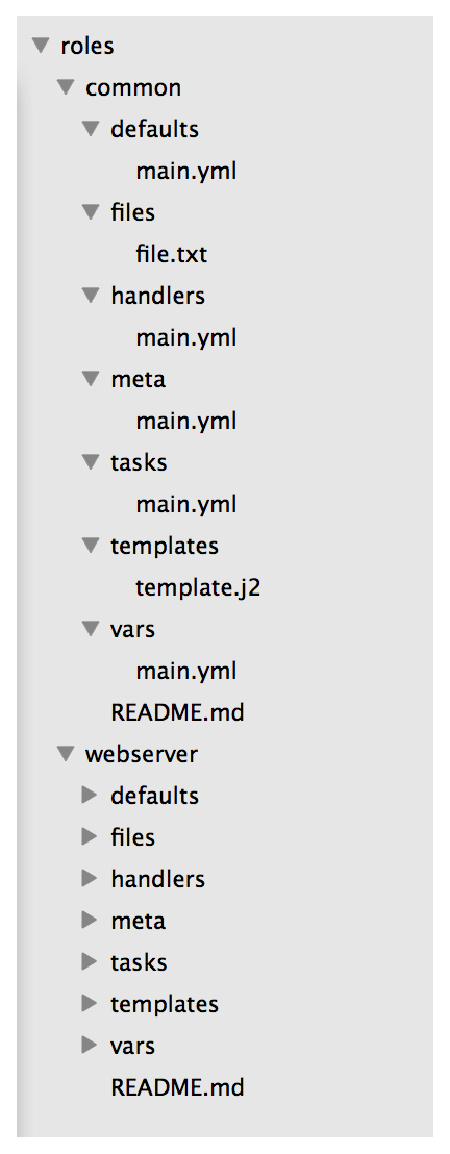
\includegraphics[width=0.35\textwidth]{figures/roles-directory.eps}
   \end{center}
   \caption{Role Directory Structure}
	\label{fig:roles}
\end{wrapfigure}

Before we go further, please refer to figure~\ref{fig:roles} on page~\pageref{fig:roles} to examine 
directory organization of roles.


 

Under each role, there are sub directories which corresponds to certain responsibility. Lets take the 
example of \emph{common} role, so when, main.yml exist under following directories:
 
 
 \begin{itemize}
\item roles/common/defaults
\item roles/common/task
\item roles/common/handlers
\item roles/common/vars
\item roles/common/meta
\end{itemize}

these files will be added to the play. Meaning you do not have to specify paths for tasks, handlers, 
variables, meta data. To make it little bit more easy, you do not have to use 
\emph{include} directives for any of these files.

When you want to use files that are under following directory, \emph{copy} and 
\emph{script} tasks will make the reference to the following directory:

\begin{itemize}
\item roles/common/files
\end{itemize}

meaning any file or script under this directory will be available copy and script tasks automatically without 
having to path them relatively or absolutely. In same matter, files located
under template directory will be available to template tasks, and files located 
under task directory will be available for include tasks.

\begin{itemize}
\item roles/common/tasks
\item roles/common/templates
\end{itemize}


\subsection{Creating Roles}
Ansible offers simple way to create complete directory structure for roles. 
Following command will create role called \emph{common} and empty YAML files in directories. 

\begin{Verbatim} 
 
ansible-galaxy init common

\end{Verbatim}


\subsection{Using Community Roles}
Ansible Galaxy, is a free site for downloading community developed Ansible 
roles, which means for most common task you do not have to write any role and 
can reuse existing role. Please refer to:
\\
\\
\url{http://galaxy.ansible.com/}



\section{Up Shot}
In this chapter we have gave brief overlook of playbook organization. 

\begin{itemize}
\item Roles : are logical directory structure which ansible knows about it and work 
 against it. It follows the method of convention over configuration. 
\end{itemize}

% ------------------------------
% End of chapter
% ------------------------------
% ------------------------------ 
% ------------------------------




% ------------------------------
% ------------------------------
% ------------------------------ 
% Beginning of a chapter
% ------------------------------

\chapter{Case Study : Multiple Playbooks}
\label{chap-multiple-playbooks}
In this chapter we will put all the things we have tried so far in previous chapters in a good 
structural way so we can take advantage of roles in Ansible.

\section{The Problem}
Here is our problem:

\begin{quote}
in \emph{\fullref{chap-common-post-installation-setup}} and 
\emph{\fullref{chap-deploying-web-application-with-nginx}}
we have made two separate tasks, which was great. However, we want to merge 
these playbooks and configure it in much more friendly way. Furthermore we want to use the playbook 
against several server with some dynamic configuration.
\end{quote}



In other words, here are the steps:
\begin{itemize}
\item Customize previous code
\item Make it installable to several server
\item Make the playbook much more dynamic
\end{itemize}


\section{The Directory Structure}
We have now two separate playbook which we want to join, one is common post 
installation and the other one is nginx installation. So what we want to do is 
make a role out of each playbook. Therefore we create the following directories first.

\begin{itemize}
\item roles/common
\item roles/webservers
\end{itemize}

If you can remember it, common post installation playbook did not include any 
templates, scripts, neither variables. So it consisted only of tasks. Nginx 
installation on the other had all these extra files. So what we will do is create 
the directory structure and add main.yml file as default to required directories:

\begin{itemize}
\item roles/common/tasks/main.yml

\item roles/webservers/files
\item roles/webservers/templates
\item roles/webservers/handlers/main.yml
\item roles/webservers/tasks/main.yml
\item roles/webservers/vars/main.yml
\end{itemize}

\section{Dividing Common Post Installation Playbook}
 Common post installation, had tasks of updating apt cache, installing ntp and 
 changing the hostname. If we want some logical structure out of it, what we can 
 do is, to separate hostname task and others. In such a case the structure of 
 the files and their content will look like this:
 
File : /roles/common/tasks/hostname.yml
\begin{Verbatim} 
 
---
 - name: Change hostname
   hostname: 
      name={{host_hostname}}

\end{Verbatim}


File : /roles/common/tasks/apt.yml
\begin{Verbatim} 
 
---
  - name : Update apt cache
    apt  : 
       update_cache=yes

  - name : apt upgrade
    apt : 
       upgrade=yes

  - name : apt dist
    apt : 
       upgrade=dist

  - name: install ntp packages
    apt:
       pkg=ntp 
       state=present

\end{Verbatim}  

And finally we can include these two files into main.yml file so by default when 
common role is executed these tasks will be included in.

File : /roles/common/tasks/main.yml
\begin{Verbatim} 
 
---
- include: hostname.yml
- include: apt.yml

\end{Verbatim}  


\section{Dividing Web Application Playbook}
In this case we have several different components which we have to place them in 
correct directories. To begin with, we need to move j2 templates to templates 
directory, and HTML and PHP files into files directory.

\begin{itemize}
\item roles/webservers/files/index.html
\item roles/webservers/files/myapp.php
\item roles/webservers/templates/default.j2
\item roles/webservers/templates/nginx.conf.j2
\end{itemize}

Next thing we can separate is handlers. So we should put our handlers under roles/webservers/handlers/main.yml


\begin{Verbatim} 
 
---
 - name: restart nginx
   service: 
      name=nginx
      state=restarted
      enabled=yes

 - name: restart php5-fpm 
   service: 
      name=php5-fpm 
      state=restarted
      enabled=yes
      
\end{Verbatim}  

As you know we also had some variables, so we can put all the variables under roles/webservers/defaults/main.yml

\begin{Verbatim} 
 
delete_default_vhost: false
user: www-data
worker_processes: 4 
pid: /var/run/nginx.pid
worker_connections: 768
httpPort: 80

\end{Verbatim}  


Only thing that is left is now to separate tasks. We will separate tasks in two 
section one is nginx installation and configuration and another one is 
deployment of the web application.

File :roles/webservers/tasks/setup\_nginx.yml
\begin{Verbatim} 
 
---
  - name: Install nginx and php-fpm 
    apt: 
       pkg="{{item}}"
       state=present
    with_items:
       - nginx
       - php5-fpm
    notify:
       - restart nginx

  - name: write nginx.conf
    template: 
       src=nginx.conf.j2
       dest=/etc/nginx/nginx.conf
    notify:
       - restart nginx

  - name: write my default site conf
    template: 
       src=default.j2
       dest=/etc/nginx/sites-enabled/default
    notify: 
       - restart nginx
       - restart php5-fpm
      
\end{Verbatim}  


File :roles/webservers/tasks/deploy\_webapp.yml
\begin{Verbatim} 
 
---
  - name: Copy files
    copy: 
       src="{{item}}"
       dest="/usr/share/nginx/www/{{item}}"
     with_items:
        - index.html 
        - myapp.php
      
\end{Verbatim} 


And finally we can include these two files into main.yml as we did before:

File :roles/webservers/tasks/main.yml
\begin{Verbatim} 
 
---
- include: setup_nginx.yml
- include: deploy_webapp.yml

\end{Verbatim}  


\section{Main Playbook}
Main playbook will be relatively small, as it only includes host definition and 
roles. This file which we will be calling \emph{webservers.yml} will be same 
directory as roles and here is the content of it:

\begin{Verbatim} 
 
- hosts: web
  sudo: true
  roles: 
    - common
    - webservers

\end{Verbatim}  

As you can see from playbook, it will run against all the host that are called 
web. And first it will execute common role and than webservers. We could 
additionaly create one more playbook in same level which only executes common 
role, because there might be cases where we may need only common post 
installation and this can run against \emph{all} servers:

\begin{Verbatim} 
 
- hosts: all
  sudo: true
  roles: 
    - common

\end{Verbatim}  

\section{Inventory File}
As one of the goal of this chapter was to run this ansible code against several 
machines, what we want to do is create a INI file which holds the hosts files. 
Here is the how host file looks like, and each host property has variable called 
\emph{host\_hostname}. This variable is used in under common post installation, 
when we change the host name. 

\begin{Verbatim} 
 
[web]
web01	ansible_ssh_host=192.168.56.150	host_hostname=web01
web02	ansible_ssh_host=192.168.56.151	host_hostname=web02
web03	ansible_ssh_host=192.168.56.152	host_hostname=web03

\end{Verbatim} 

 % ---- NOTE BEGINS ---- 
\begin{mdframed}[style=noteStyle]
\begin{minipage}[b]{0.05\textwidth}
\begin{figure}[H]

\includegraphics[width=0.9\textwidth]{figures/notes-icon.eps} 
\end{figure}
\end{minipage}  
\begin{minipage}[b]{0.05\textwidth}
\textbf{Note}
\end{minipage}

If you are using vagrant file that we have provided you can increase number of servers 
by increasing a variable in vagrant file. For details please refer 
to \emph{Appendix \fullref{appendix:installing-and-using-vagrant}}
\end{mdframed}
 % ---- NOTE ENDS ---- 



\section{Executing Playbook}
You can execute the playbook same way as we have done before, however this time instead of giving 
server address, we can specify inventory file: 

\begin{Verbatim} 
 
ansible-playbook -i hosts.ini webservers.yml 

\end{Verbatim} 

This will execute webservers role for all three servers.

\section{Up Shot}
In this chapter we have illustrated how you can organize playbooks by seperating tasks, variables, handlers 
as well as running a playbook against several servers.

% ------------------------------
% End of chapter
% ------------------------------
% ------------------------------ 
% ------------------------------











% ------------------------------
% ------------------------------
% ------------------------------ 
% Beginning of a chapter
% ------------------------------

\chapter{Case Study : Ansible Configuration}
\label{chapter:ansible-configuration}
Until this chapter, every single example we have made was with out-of-box 
configuration. However there will be times, for example next chapter, 
where you need to change the default configuration to control ansible' work 
flow. In this chapter we will give small hints regarding ansible configuration 
and how can it be changed to fit in your workflow.


\section{ansible.cfg File}
 When ansible runs, it loads bunch of configuration parameter from a file called \emph{ansible.cfg}.
 This is an INI file, which content of it looks like this:
 
 
 \begin{verbatim}
 
...

[defaults]

# some basic default values...

hostfile       = /etc/ansible/hosts
library        = /usr/share/ansible
remote_tmp     = $HOME/.ansible/tmp
pattern        = *
forks          = 5
poll_interval  = 15
sudo_user      = root
#ask_sudo_pass = True
#ask_pass      = True
transport      = smart
remote_port    = 22
....

 \end{verbatim}
 

The example above is only small part of a configuration of ansible. We will not 
explain every single parameter that can be configured, but we will give some 
important tips about how it can make your life much more easier.

\subsection{Config File Location and Order}
Ansible offers relatively easy way to configure it self. You could load 
configuration from different location as well as as Environment Variable. By 
default configuration is sane, so you will probably not need to change a lot. 
However in case if you have to, we will show you how to do it.

To begin with, ansible can load the configuration file from following 
directories in respected order. First configuration file that is found will be 
used.

\begin{itemize}
\item ANSIBLE\_CONFIG : This is a environment variable that points to a configuration file. It might be helpful
for dynamically loading configuration file.

\item  CWD : Current working directory, this might be useful for some 
configuration belongs to certain playbooks.

\item HOME : User home directory, this might be useful for some 
configuration that belongs only to you. Settings in here might be much more 
generic and not so much of server related configuration. Ansible looks for the \emph{.ansible.cfg} 
file.

\item /etc/ansible/ansible.cfg : Those configuration that are used system wide can be placed in 
this location.
\end{itemize}


\subsection{Loading and Using Configuration}
Ansible does not discard all the default variables when it loads a configuration file. 
For instance, if you put the following configuration file in your working 
directory and execute the \emph{ansible}, what will happen is, ansible will load 
the configuration file and it will overwrite only default module name and 
everything else will be the same.

\begin{verbatim}

[defaults]
module_name    = ping

\end{verbatim}

You can test this with following command, add the configuration file in a 
directory, and open it in your terminal, when you execute the following command 
you can see the it uses \emph{ping} module as default module.

\begin{verbatim}

ansible -i 192.168.56.150,  all

\end{verbatim}



\section{Environment Variables}
You could also set some of the configuration via environment variables. Because 
environment variables has the highest precedence it will be used by the ansible 
instead of other variables that are set in your configuration file. For instance 
when you are using roles, and you want your roles to be in a single directory, 
one of the best way to manage them is to set \emph{ANSIBLE\_ROLES\_PATH} variable. 
By default this is set to \emph{/etc/ansible/roles}. Soon as you change this 
value, all roles will be installed(via ansible-galaxy) to directory you have set 
and when ansible looks for roles it will checkout the directory you have 
specified to find out whether roles are located under there or not. 

\subsection{Examples}
\subsubsection{Multiple Role Directories}
To begin with, here is simply how you can set the environment variable for 
roles.

\begin{verbatim}
  
  export ANSIBLE_ROLES_PATH=path/to/your/roles
  
\end{verbatim}

Another possibility which is also might help you is to have multiple directories 
for roles, you might use this for public(open-source) and private roles, which might be the 
case if you are not allowed to disclose some of your roles. In following example, 
we give two directories to the \emph{export} build-in command. Which means 
ansible will look under both directories for roles.

\begin{verbatim}
  
  export ANSIBLE_ROLES_PATH=/path/to/your/roles/public:/path/to/your/roles/private
   
\end{verbatim}


 % ---- NOTE BEGINS ---- 
\begin{mdframed}[style=noteStyle]
\begin{minipage}[b]{0.05\textwidth}
\begin{figure}[H]

\includegraphics[width=0.9\textwidth]{figures/notes-icon.eps} 
\end{figure}
\end{minipage}  
\begin{minipage}[b]{0.05\textwidth}
\textbf{Note}
\end{minipage}

Environment variables are not persistent, once the session is terminated the 
values that you have set will be lost. Therefore, if you want to make it 
persistent you have to add that in to your bash profile. You can find your bash 
profile under your home directory  \emph{~/.bash\_profile}
\end{mdframed}
 % ---- NOTE ENDS ---- 
 
 

\subsubsection{Host Files}
TBA

\begin{verbatim}
  
  export ANSIBLE_HOSTS=/path/to/inventory
   
\end{verbatim}



\subsubsection{Logging}
In case if you want to activate logging, you can either add a location for you 
log files into your ansible configuration file or you can add an environment 
variable. Following example, will allow ansibe to generate a log file under defined directory, 
based on date. When ansible notices this log directory it will log information about executions at the designated 
location.

\begin{verbatim}
  
  export ANSIBLE_LOG_PATH=/path/to/your/logs/ansible-$(date '+%Y-%m-%d').log
   
\end{verbatim}



\section{Additional Information}
In following URLs you can find additional information regarding ansible 
configuration. Following links points to python file that is used in ansible, 
which can give you an insight to configuration and values that are exist.

\url{https://github.com/ansible/ansible/blob/devel/lib/ansible/constants.py}

Following link is from ansible website, which is a detailed information about 
what kind of arguments can be configured and what they are used for.

\url{http://docs.ansible.com/intro_configuration.html}



\section{Up Shot}
TBA

% ------------------------------
% End of chapter
% ------------------------------
% ------------------------------ 
% ------------------------------

 
 
% ------------------------------
% END OF THE BOOK
% ------------------------------
% ------------------------------ 
% ------------------------------

\printindex

\clearemptydoublepage
%\blankpage
%\blankpage
%\blankpage


\begin{appendices}
\chapter{How to Install Ansible}
\label{appendix:How-to-install-ansible}
Installing Ansible is relatively easy, most likely the best way is to checkout the repository 
and start using it. With this approach you can just pull latest changes and you 
can use the features immediately. But other methods are just fine as well. 

\section{Install From Source Code}
 To install Ansible from source:
 
\begin{Verbatim}

$ git clone git://github.com/ansible/ansible.git
$ cd ./ansible
$ source ./hacking/env-setup
  
\end{Verbatim}

There are several dependency which you can install via python package manager, 
\emph{pip}. If you don't have the pip first install pip:

\begin{Verbatim}
  
$ sudo easy_install pip

\end{Verbatim}

Ansible also uses the following Python modules that need to be installed:

\begin{Verbatim}

$ sudo pip install paramiko PyYAML jinja2 httplib2
  
\end{Verbatim}

\section{Install via Package Manager}
Alternatively you can install via package manager that you are using:

via homebrew :

\begin{Verbatim}

$ brew install ansible

\end{Verbatim}

via pip:

\begin{Verbatim}

$ sudo pip install ansible

\end{Verbatim}

via apt

\begin{Verbatim}

$ sudo apt install ansible

\end{Verbatim}

via yum

\begin{Verbatim}

$ sudo yum install ansible

\end{Verbatim}


via pkg

\begin{Verbatim}

$ sudo pkg install ansible

\end{Verbatim}

If you have any installation problems please refer to:

\url{http://docs.ansible.com/intro_installation.html}


\chapter{Installing and Using Vagrant }
\label{appendix:installing-and-using-vagrant}
Vagrant is a tool for creating, configuring, managing virtual 
machines. Because we want you to actually test the things we have shown in this 
book, we have prepared a simple Vagrant file which you can use 
for firing one or several virtual machines quickly. Furtheremore, we have add a 
small playbook which will copy your public SSH key into vagrant machine so you 
don't have to do anything.


\section{Requirements}
To use vagrant you need to install vagrant and virtualbox, please download both 
and install it.

\begin{itemize}
\item \url{http://www.vagrantup.com/}
\item \url{http://www.virtualbox.org/}
\end{itemize}

You also need a SSH key, we assume that your SSH keys under your home directory. In MacOS this should be:

\begin{verbatim}

/Users/adham/.ssh/id_rsa.pub

   
\end{verbatim}

If you don't have a SSH key, please create one and then proceed.


\section{Starting Vagrant Machine}
To create a vagrant machine, open your terminal, go to 
\emph{source-code/Appendix B - Installing and Using Vagrant} folder, and 
execute following command.

\begin{verbatim}
  
  vagrant up

\end{verbatim}

This command will create a new vagrant machine and will copy your public SSH key. 
By default first machine that is created will have the following IP address:

\begin{verbatim}
  
192.168.56.150

\end{verbatim}

For more information about how to use vagrant please refer to:

\url{http://docs.vagrantup.com/}


\section{Increasing Number of Machines}
If you want to increase the number of machines that you are firing-up you can 
simply increas the \emph{nodes} value in vagrant file. You can also change the 
default IP address.


\section{Vagrant and Ansible Code}
We have an ansible playbook which creates local user and copy SSH key. Here is the content of vagrant file:

\begin{verbatim}

Vagrant.configure("2") do |config|
  config.vm.box_url = "http://files.vagrantup.com/precise64.box"

  ## Nodes
  nodes =1
  rangeofips = 149
  (1..nodes).each do |n|
     
    vmip   = "192.168.56.#{rangeofips + n.to_i}"
    name = "vagrant0#{n}.local"
    puts "Let's talk about %s." % name
    ## Node Conf
    config.vm.define name do |cfg|
      cfg.vm.box = name
      cfg.vm.host_name = name
      ## Comment public network to disable bridge
      cfg.vm.network :public_network
      cfg.vm.network :private_network, ip: vmip
	    cfg.ssh.forward_agent = true
	    cfg.vm.provider "virtualbox" do |vb|
        ## headless or non headless machine
        vb.gui = false
      end

      ## Ansible Provisioning
      cfg.vm.provision :ansible do |ansible|
 	      ansible.playbook = "vagrant-provision.yml"
	      ## Debugging
    	  ansible.verbose =  true
	      ansible.verbose="vvvvv"
      end
    end
  end
end

\end{verbatim}


And here is the ansible code:

\begin{verbatim}
  
  ---
#
# This playbook deploys your keys to the vagrant
#

- name: Provision my keys
  hosts: all
  sudo: True
  vars:
    localuser: "{{ lookup('ENV','USER') }}"
    mypassword : "$5$rounds=110000$Jm.keFgd6zfXrnvJ$ar4ns4Y/Vds32qqet19KlR3evMgRkdTjoIf3eL7zBd7" ## password is vagrant only creates password if you dont have keys
  tasks:
    - name: Create your local user
      user:
        name="{{localuser}}"
        home="/home/{{localuser}}"
        shell="/bin/bash"
        append="true"
        group="admin"
        comment="{{localuser}}"

    - name: check keys
      stat:
         path="~/.ssh/id_rsa.pub"
         get_md5=no
         follow=yes
      register: mypubkey
      sudo_user: "{{localuser}}"
      connection: local

    - name: Putting you authorized_key
      authorized_key:
        key="{{lookup('file', '~/.ssh/id_rsa.pub')}}"
        user="{{localuser}}"
        manage_dir=yes
      when: "mypubkey.stat.exists == True"

    - name: Create password as you are not using keys
      user:
        name="{{localuser}}"
        password="{{mypassword}}"
      when: "mypubkey.stat.exists == False"
      
\end{verbatim}

\end{appendices}



\end{document}
